\documentclass{beamer}

\renewcommand\sfdefault{phv}
\renewcommand\familydefault{\sfdefault}
\usetheme{default}
\usepackage{color}
\useoutertheme{default}
\usepackage{texnansi}
\usepackage{color}
\usepackage{marvosym}
\definecolor{bottomcolour}{rgb}{0.32,0.3,0.38}
\definecolor{middlecolour}{rgb}{0.08,0.08,0.16}
\setbeamerfont{title}{size=\Huge}
\setbeamercolor{structure}{fg=gray}
\setbeamertemplate{frametitle}[default]%[center]
\setbeamercolor{normal text}{bg=black, fg=white}
\setbeamertemplate{background canvas}[vertical shading]
[bottom=bottomcolour, middle=middlecolour, top=black]
\setbeamertemplate{items}[circle]
\setbeamerfont{frametitle}{size=\huge}
\setbeamertemplate{navigation symbols}{} %no nav symbols


\usepackage{amsmath,  amsfonts, amsthm, graphicx, subfigure}
%\usepackage{biblatex}
 \usepackage{fancybox, ulem}
 \usepackage{mathtools}
 \usepackage{tabularx}
 \usepackage{tikz}
 \usepackage{movie15}
 %\bibliography{pumping_paper}
\newcommand{\p}{\partial}
\newcommand{\f}{\frac}
\newcommand{\B}{\textbf}
\newcommand{\I}{\textit}

 % \usetheme{Singapore}
% \usetheme{Warsaw}
  \setbeamertemplate{navigation symbols}{}
\title{ Matlab Notes Part 1}
\author{Austin Baird\\UNC Department of Mathematics\\UNC Department of Biology}
\date{\today} 

\begin{document}
\frame{\titlepage}

\begin{frame}
\frametitle{Introduction}
\begin{itemize}
\item Matlab is a lot like a calculator! 
\item we can compute things like $ 3\cdot 2$ 
\item Arithmetic is preformed in order of operations (just like a calculator) 
\item Matrices and matrix operations are where Matlab excels
\item Today we will: 
\begin{itemize}
\item Understand the basic Desktop environment
\item Preform basic arithmetic
\item use built in functions
\item Create matices and write our first code
\end{itemize}

\end{itemize}
\end{frame}

%--------------------------------------------------------------------------------------------------------------------------------------------------------------------------------------------------------------------------%
\begin{frame}
\frametitle{Desktop Basics} 

\begin{figure}
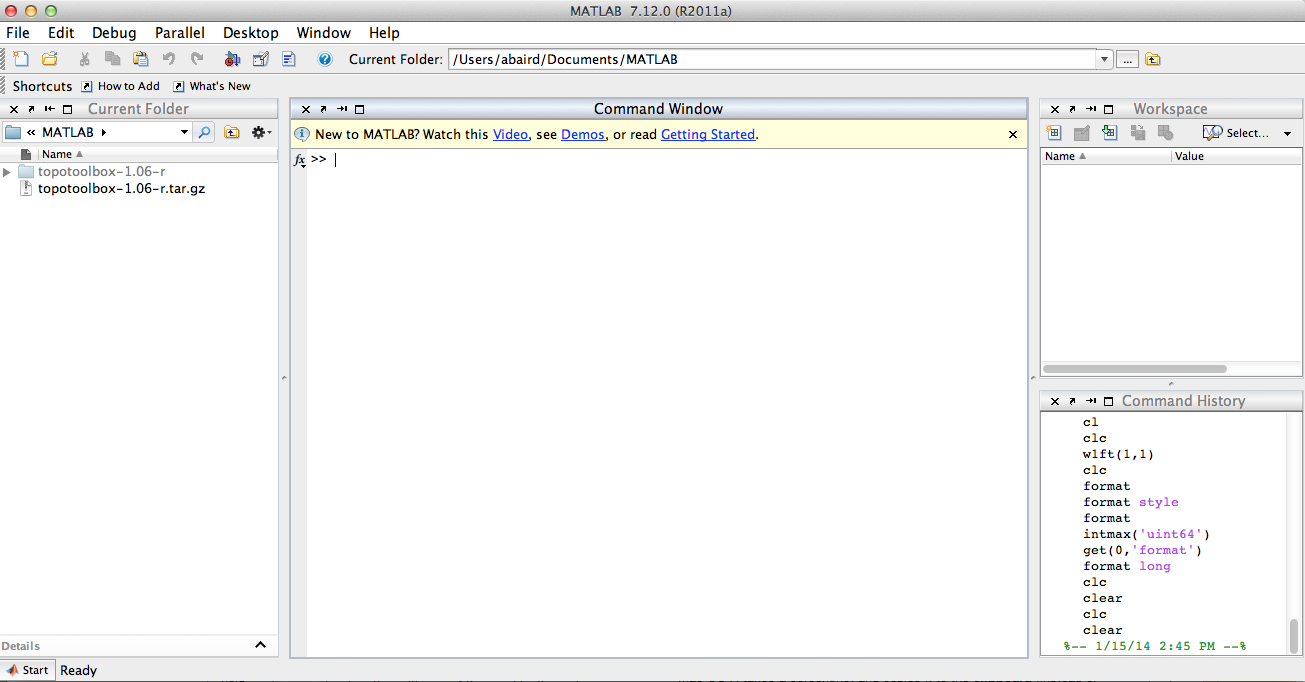
\includegraphics[width=\textwidth, height= 0.8\textheight]{./pictures/display}
\end{figure}
\end{frame}

%--------------------------------------------------------------------------------------------------------------------------------------------------------------------------------------------------------------------------%

\begin{frame}
\frametitle{Desktop Basics} 
\begin{itemize}
\item \B{Current Folder}: This is where the files you are working with will be stored. Note: you can navigate from the folder you're in to any folder you desire by clicking the magnifying glass. 
\item \B{Command Window}: This is where you can calculate, receive error messages, or print output from your programs. Commands are input at the $\gg$ symbol. 
\begin{itemize}
\item try to calculate things right now! 
\end{itemize}
\item \B{Workspace:} This is where variables are stored and will tell you things about them (what they equal, how big a matrix is ect.)
\item \B{Command History:} This is where the commands you've issued most recently will appear. $\uparrow$ on your keyboard will scroll through these commands. 
\item Refer to the text (Matlab intro) for more detailed instruction.
\end{itemize}

\end{frame}

%--------------------------------------------------------------------------------------------------------------------------------------------------------------------------------------------------------------------------%

\begin{frame}
\frametitle{Troubleshooting} 

\begin{itemize}
\item Often times things won't work. 
\item One \B{Common} problem is that a variable you thought was free is actually associated with a value. 
\item Try the command $\gg$ clear. This will clear all the variables in the \B{Workspace}. 
\end{itemize}

\LARGE 
Try and do some computing and assign variables to values. 

\end{frame}

%--------------------------------------------------------------------------------------------------------------------------------------------------------------------------------------------------------------------------%

\begin{frame}
\frametitle{Arrays} 
\begin{itemize} 
\item Matlab = Matrix Laboratory, so do things with matrices! 
\item Create your first matrix! 
\begin{itemize}
\item $\gg a = [1 2 3 4]$, Row Vector! 
\item Indexing in matlab begins with 1 (\B{NOT} 0) 
\item Add more rows: $\gg a = [1 2 3 4; 2 3 4 5; 3 4 5 6]$
\item \B{Note} This also works: $\gg a = [1,2,3,4;2,3,4,5;3,4,5,6]$
\item We can call values from this array: 
\item $\gg a(1,2)$
\item $\gg 2$ 
\item Or assign a value to a particular position: 
\item $\gg a(1,2)=10$  
\item The notation is (row, column)
\end{itemize}


\end{itemize} 
\end{frame}



%--------------------------------------------------------------------------------------------------------------------------------------------------------------------------------------------------------------------------%

\begin{frame}
\frametitle{Array Creating Functions}

\begin{itemize}
\item There are ways to automatically create an array(matrix) in matlab:
\begin{itemize}
\item $\gg a = zeros(3,2)$ 
\item Creates an array of all zeros (this is good for data management if you want a set size for your matrix
\item $\gg a = linspace(0,1,100)$ 
\item This creates a vector which has 100 points filled in between 0 and 1. 
\item $\gg a = 0:0.1:1$ 
\item this creates an array which has mesh width equal to 0.1 
\end{itemize}
\item How do we model functions in Matlab? 
\end{itemize}



\end{frame} 


%--------------------------------------------------------------------------------------------------------------------------------------------------------------------------------------------------------------------------%


\begin{frame}
\frametitle{Array Operations} 

\begin{itemize} 
\item Colon operator:
\item $\gg a = [1 2 3 ; 2 3 4 ; 4 5 6]$
\item The colon denotes \I{start}:\I{end}. \I{Note:} if you just place a colon it will select everything.
\item Select the first two rows of our matrix: 
\begin{itemize}
\item $\gg a(1:2, :)$
\item  What does $ \gg a(1,:)$ do? 
\end{itemize}
\item We can also add to each element of the array: 
\begin{itemize}
\item $\gg a -a $ 
\item $\gg a - 10 $ 
\end{itemize}
\item We can do traditional and element wise multiplication of matrices: 
\begin{itemize}
\item traditional: $\gg a*a$, element wise: $\gg a.*a$
\item In a similar way you can do other things element wise to a matrix ex.: $\gg a.\wedge 3$
\end{itemize}
\end{itemize}
\end{frame}
%--------------------------------------------------------------------------------------------------------------------------------------------------------------------------------------------------------------------------%

\begin{frame}
\frametitle{Discrete Functions} 
\begin{itemize}
\item In math things are continuous, in Matlab (and in computational science in general) This is not the case. 
\item To compute and evaluate functions we need a \I{Domain} and their corresponding function values \I{Range}
\item To get a Domain in Matlab we must ``discretize'' our continuous domain. 
\item We do this by creating a ``mesh width'' = size of our spacing in our discretization
\begin{itemize}
\item ex: $\gg x = linspace(0,1,10)$ what is our mesh width $dx$ (x(2)-x(1))? is it always equal? Must consider this!  
\item ex: $\gg x = 0:0.1:1$ what is our mesh width $dx$? 
\end{itemize}

\end{itemize}

\end{frame}

%--------------------------------------------------------------------------------------------------------------------------------------------------------------------------------------------------------------------------%

\begin{frame}
\frametitle{Evaluating Functions} 
\begin{itemize}
\item Now that we have a discretized version of the x-axis we can now evaluate a function! 
\item Matlab has many built in functions (sin, cos, tan, exp...)
\item $\gg y = sin(x) $ 
\item We now have a set of range values, how do we know that this is right? Graph? 
\item plot this function: $ \gg plot(y) $
\item In general the resolution of our function is dependent upon our mesh width
\item How small is enough, how big is too big? Does any mesh width work? 
\item A quick and dirty estimate of the error between two arrays: $max(a - b )$ will select the max error between the arrays (infinity norm). 
\item Plot sin over one period and experiment with different mesh widths and their effects
\end{itemize}

\end{frame}


%--------------------------------------------------------------------------------------------------------------------------------------------------------------------------------------------------------------------------%

\begin{frame}
\frametitle{ Our First Program} 
\begin{itemize}
\item Matlab files are denoted by a .m at the end of the name.
\item Documentation is very very important! \% is how you comment lines (these will not be read by the computer) 
\item Notice that to run the code Matlab asks you whether to add folder to path or to change to directory, both work. 
\item Just type the name of the code in the command line to get the program to run. 
\end{itemize}

\end{frame}

%--------------------------------------------------------------------------------------------------------------------------------------------------------------------------------------------------------------------------%


\begin{frame}
\frametitle{How to Run} 

\begin{figure}
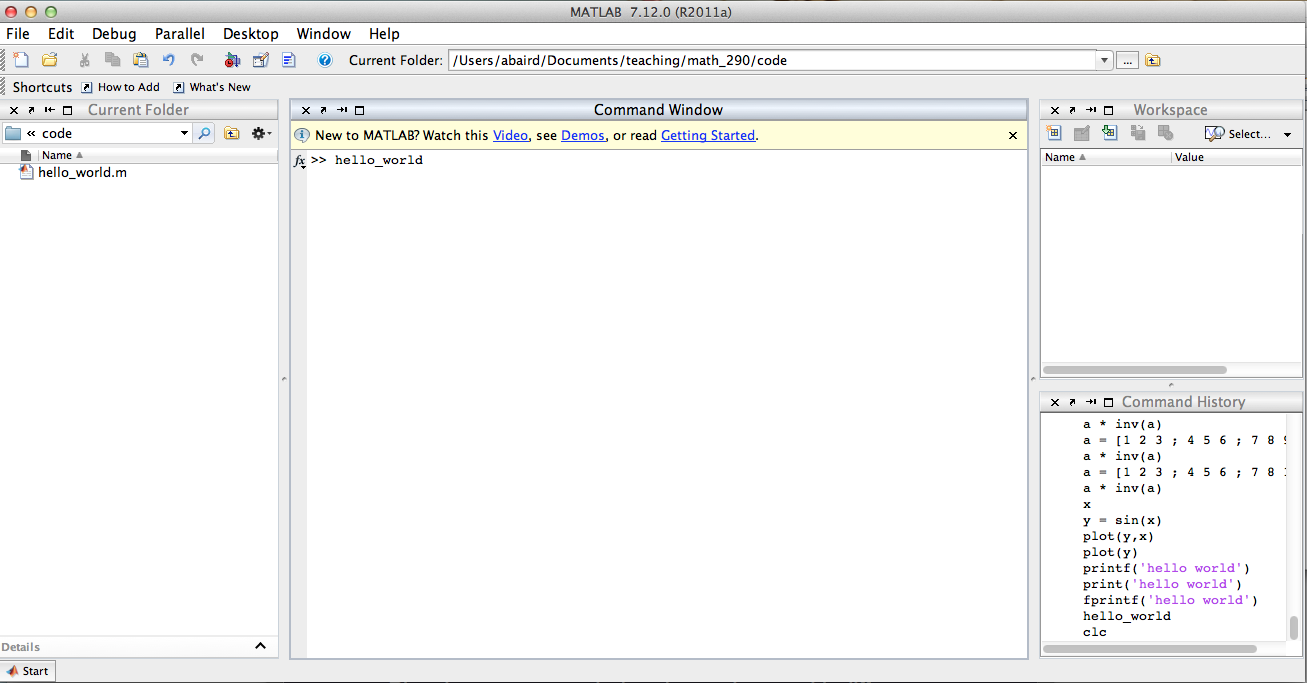
\includegraphics[width=\textwidth, height= 0.8\textheight]{./pictures/hello_world}
\end{figure}
\end{frame}


%--------------------------------------------------------------------------------------------------------------------------------------------------------------------------------------------------------------------------%
\begin{frame}
\frametitle{Output} 

\begin{figure}
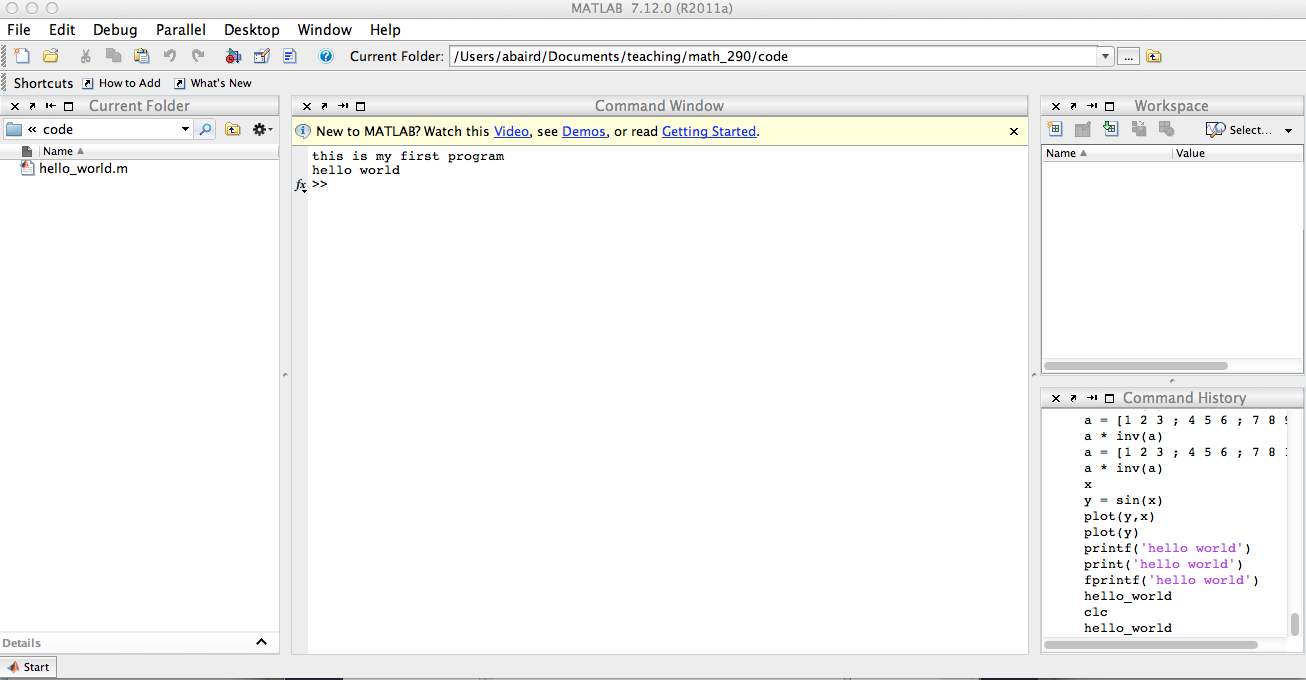
\includegraphics[width=\textwidth, height= 0.8\textheight]{./pictures/output}
\end{figure}
\end{frame}

%--------------------------------------------------------------------------------------------------------------------------------------------------------------------------------------------------------------------------%


\begin{frame}

\frametitle{Homework} 
\begin{itemize} 
\item Read sections 1-17 to 1-23
\item Email me by Tuesday at 12:01am a onyen.m file which when run does the following ( and is commented at the top of the file with your full name and who you worked with, if anyone): 
\begin{itemize}
\item Generates a figure which plots $ y = sin(x)+c$ for \I{ten} values of c (all on the same figure). 
\item Generates the figure in section 1-23.
\end{itemize}
\end{itemize}

\end{frame}
\end{document}
